% ========================================
%	Header einbinden
% ========================================

\documentclass[bibtotoc,titlepage]{scrartcl}

% Deutsche Spracheinstellungen
\usepackage[ngerman,german]{babel, varioref}
\usepackage[T1]{fontenc}
\usepackage[utf8]{inputenc}

%\usepackage{marvosym}

\usepackage{amsfonts}
\usepackage{amssymb}
\usepackage{amsmath}
\usepackage{amscd}
\usepackage{amstext}
\usepackage{float}
\usepackage{caption}
\usepackage{wrapfig}
\usepackage{setspace}
\usepackage{threeparttable}
\usepackage{footnote}

\usepackage{caption}
\usepackage{subcaption}

\newfloat{formel}{htbp}{for}
\floatname{formel}{Formel}


\usepackage{longtable}

%\usepackage{bibgerm}

\usepackage{footnpag}

\usepackage{ifthen}                 %%% package for conditionals in TeX
\usepackage{siunitx}
%Fr textumflossene Bilder und Tablellen
%\usepackage{floatflt} - veraltet

%Fr Testzwecke aktivieren, zeigt labels und refs im Text an.
%\usepackage{showkeys}

% Abstand zwischen zwei Abs�zen nach DIN (1,5 Zeilen)
% \setlength{\parskip}{1.5ex plus0.5ex minus0.5ex}

% Einrckung am Anfang eines neuen Absatzes nach DIN (keine)
%\setlength{\parindent}{0pt}

% R�der definieren
% \setlength{\oddsidemargin}{0.3cm}
% \setlength{\textwidth}{15.6cm}

% bessere Bildunterschriften
%\usepackage[center]{caption2}


% Probleml�ungen beim Umgang mit Gleitumgebungen
\usepackage{float}

% Nummeriert bis zur Strukturstufe 3 (also <section>, <subsection> und <subsubsection>)
%\setcounter{secnumdepth}{3}

% Fhrt das Inhaltsverzeichnis bis zur Strukturstufe 3
%\setcounter{tocdepth}{3}

\usepackage{exscale}

\newenvironment{dsm} {\begin{displaymath}} {\end{displaymath}}
\newenvironment{vars} {\begin{center}\scriptsize} {\normalsize \end{center}}


\newcommand {\en} {\varepsilon_0}               % Epsilon-Null aus der Elektrodynamik
\newcommand {\lap} {\; \mathbf{\Delta}}         % Laplace-Operator
\newcommand {\R} { \mathbb{R} }                 % Menge der reellen Zahlen
\newcommand {\e} { \ \mathbf{e} }               % Eulersche Zahl
\renewcommand {\i} { \mathbf{i} }               % komplexe Zahl i
\newcommand {\N} { \mathbb{N} }                 % Menge der nat. Zahlen
\newcommand {\C} { \mathbb{C} }                 % Menge der kompl. Zahlen
\newcommand {\Z} { \mathbb{Z} }                 % Menge der kompl. Zahlen
\newcommand {\limi}[1]{\lim_{#1 \rightarrow \infty}} % Limes unendlich
\newcommand {\sumi}[1]{\sum_{#1=0}^\infty}
\newcommand {\rot} {\; \mathrm{rot} \,}         % Rotation
\newcommand {\grad} {\; \mathrm{grad} \,}       % Gradient
\newcommand {\dive} {\; \mathrm{div} \,}        % Divergenz
\newcommand {\dx} {\; \mathrm{d} }              % Differential d
\newcommand {\cotanh} {\; \mathrm{cotanh} \,}   %Cotangenshyperbolicus
\newcommand {\asinh} {\; \mathrm{areasinh} \,}  %Area-Sinus-Hyp.
\newcommand {\acosh} {\; \mathrm{areacosh} \,}  %Area-Cosinus-H.
\newcommand {\atanh} {\; \mathrm{areatanh} \,}  %Area Tangens-H.
\newcommand {\acoth} {\; \mathrm{areacoth} \,}  % Area-cotangens
\newcommand {\Sp} {\; \mathrm{Sp} \,}
\newcommand {\mbe} {\stackrel{\text{!}}{=}}     %Must Be Equal
\newcommand{\qed} { \hfill $\square$\\}
\renewcommand{\i} {\imath}
\def\captionsngerman{\def\figurename{\textbf{Abb.}}}

%%%%%%%%%%%%%%%%%%%%%%%%%%%%%%%%%%%%%%%%%%%%%%%%%%%%%%%%%%%%%%%%%%%%%%%%%%%%
% SWITCH FOR PDFLATEX or LATEX
%%%%%%%%%%%%%%%%%%%%%%%%%%%%%%%%%%%%%%%%%%%%%%%%%%%%%%%%%%%%%%%%%%%%%%%%%%%%
%%%
\ifx\pdfoutput\undefined %%%%%%%%%%%%%%%%%%%%%%%%%%%%%%%%%%%%%%%%% LATEX %%%
%%%
\usepackage[dvips]{graphicx}       %%% graphics for dvips
\DeclareGraphicsExtensions{.eps,.ps}   %%% standard extension for included graphics
\usepackage[ps2pdf]{thumbpdf}      %%% thumbnails for ps2pdf
\usepackage[ps2pdf,                %%% hyper-references for ps2pdf
bookmarks=true,%                   %%% generate bookmarks ...
bookmarksnumbered=true,%           %%% ... with numbers
hypertexnames=false,%              %%% needed for correct links to figures !!!
breaklinks=true,%                  %%% breaks lines, but links are very small
linkbordercolor={0 0 1},%          %%% blue frames around links
pdfborder={0 0 112.0}]{hyperref}%  %%% border-width of frames
%                                      will be multiplied with 0.009 by ps2pdf
%
%\hypersetup{ pdfauthor   = {Hannes Franke; Julius Tilly},
%pdftitle    = {x}, pdfsubject  = {Protokoll FP}, pdfkeywords = {V301, Innenwiderstand, Leistungsanpassung},
%pdfcreator  = {LaTeX with hyperref package}, pdfproducer = {dvips
%+ ps2pdf} }
%%%
\else %%%%%%%%%%%%%%%%%%%%%%%%%%%%%%%%%%%%%%%%%%%%%%%%%%%%%%%%%% PDFLATEX %%%
%%%
\usepackage[pdftex]{graphicx}      %%% graphics for pdfLaTeX
\DeclareGraphicsExtensions{.pdf}   %%% standard extension for included graphics
\usepackage[pdftex]{thumbpdf}      %%% thumbnails for pdflatex
\usepackage[pdftex,                %%% hyper-references for pdflatex
bookmarks=true,%                   %%% generate bookmarks ...
bookmarksnumbered=true,%           %%% ... with numbers
hypertexnames=false,%              %%% needed for correct links to figures !!!
breaklinks=true,%                  %%% break links if exceeding a single line
linkbordercolor={0 0 1},
linktocpage]{hyperref} %%% blue frames around links
%                                  %%% pdfborder={0 0 1} is the default
% \hypersetup{
% pdftitle    = {V301 Innenwiderstand und Leistungsanpassung}, 
% pdfsubject  = {Protokoll AP}, 
% pdfkeywords = {V301, Innenwiderstand, Leistungsanpassung},
% pdfsubject  = {Protokoll AP},
% pdfkeywords = {V301, Innenwiderstand, Leistungsanpassung}}
%                                  %%% pdfcreator, pdfproducer,
%                                      and CreationDate are automatically set
%                                      by pdflatex !!!
\pdfadjustspacing=1                %%% force LaTeX-like character spacing
\usepackage{epstopdf}
%
\fi %%%%%%%%%%%%%%%%%%%%%%%%%%%%%%%%%%%%%%%%%%%%%%%%%%% END OF CONDITION %%%
%%%%%%%%%%%%%%%%%%%%%%%%%%%%%%%%%%%%%%%%%%%%%%%%%%%%%%%%%%%%%%%%%%%%%%%%%%%%
% seitliche Tabellen und Abbildungen
%\usepackage{rotating}
\usepackage{ae}
\usepackage{
  array,
  booktabs,
  dcolumn
}
\makeatletter 
  \renewenvironment{figure}[1][] {% 
    \ifthenelse{\equal{#1}{}}{% 
      \@float{figure} 
    }{% 
      \@float{figure}[#1]% 
    }% 
    \centering 
  }{% 
    \end@float 
  } 
  \makeatother 


  \makeatletter 
  \renewenvironment{table}[1][] {% 
    \ifthenelse{\equal{#1}{}}{% 
      \@float{table} 
    }{% 
      \@float{table}[#1]% 
    }% 
    \centering 
  }{% 
    \end@float 
  } 
  \makeatother 
%\usepackage{listings}
%\lstloadlanguages{[Visual]Basic}
%\allowdisplaybreaks[1]
%\usepackage{hycap}
%\usepackage{fancyunits}

% ========================================
%	Angaben für das Titelblatt
% ========================================

\title{V01: Lebensdauer der Myonen\\				% Titel des Versuchs 
	\large TU Dortmund, Fakultät Physik\\ 
	\normalsize Fortgeschrittenen-Praktikum}

\author{Jan Adam\\			% Name Praktikumspartner A
	{\small \href{jan.adam@tu-dortmund.de}{jan.adam@tu-dortmund.de}}	% Erzeugt interaktiven einen Link
	\and						% um einen weiteren Author hinzuzfügen
	Felix Wieland\\					% Name Praktikumspartner B
	{\small \href{felix.wieland@tu-dortmund.de}{felix.wieland@tu-dortmund.de}}		% Erzeugt interaktiven einen Link
}
\date{20.06.2016}				% Das Datum der Versuchsdurchführung

% ========================================
%	Das Dokument beginnt
% ========================================

\begin{document}
	
% ========================================
%	Titelblatt erzeugen
% ========================================

\maketitle					% Jetzt wird die Titelseite erzeugt
\thispagestyle{empty} 				% Weder Kopfzeile noch Fußzeile

% ========================================
%	Der Vorspann
% ========================================

\tableofcontents
\newpage					% eine neue Seite

% ========================================
%	Kapitel
% ========================================
\section{Ziel}
Ziel dieses Versuches ist es die mittlere Lebensdauer kosmischer Myonen zu messen.

\section{Theoretische Grundlagen}
\subsection{Grundlegende Bemerkungen}
Gemäß dem Standard Modell lassen sich die elementaren Teilchen in zwei Gruppen aufteilen, für die jeweils die starke Wechselwirkung gilt (Quarks) bzw. nicht gilt (Leptonen). Myonen $\mu^-$ gehören zur zweiten Generation der Leptonenfamilie, da sie im Bezug auf ihre Masse zwischen den leichteren Elektronen $\textrm{e}^-$ und den schwereren Tauonen $\tau^-$ liegen, wobei für die Massen gilt

\begin{align}
\textrm{m}_\mu = 206,77 \textrm{m}_{\textrm{e}} = \frac{1}{3491}\textrm{m}_{\tau}\;.
\end{align}

Aufgrund ihrer Ladung wechselwirken diese Teilchen elektromagnetisch mit ihrer Umgebung. Elektronen sind als einzige dieser drei Teilchen stabil, während Myonen und Tauonen eine endliche Lebensdauer haben. Da alle Leptonen Fermionen sind, gehorchen diese Teilchen der Fermi-Dirac Statistik und besitzen eine Spin von 1/2. Des Weiteren existieren neben den bereits genannten Teilchen noch die zugehörigen Antiteilchen und die Neutrinos für jede Leptonengeneration.

Myonen entstehen u.A. in der oberen Atmosphäre aus dem Zerfall von Pionen, die zuvor aus der Wechselwirkung von energiereichen Protonen der Höhenstrahlung mit Atomkernen der Luftmolekülen entstanden sind:

\begin{align}
\pi^+ \longrightarrow &\; \mu^+ + \nu_\mu \\
\pi^- \longrightarrow &\; \mu^- + \overline{\nu}_\mu 
\end{align}

\subsection{Die Lebensdauer $\tau$}
Der Zerfall instabiler Teilchen ist ein statistischer Prozess und die Lebensdauer $\tau$ stellt eine charakteristische Größe zur Beschreibung instabiler Teilchen dar. Die Wahrscheinlichkeit $dW$ für den Eintritt eines Zerfalls lässt sich schreiben als
 
\begin{align}
dW = \lambda dt \;, \label{eqn:WSK}
\end{align}

wobei der Zusammenhang zwischen der Konstante $\lambda$ und der Lebensdauer weiter unten hergestellt wird. Aus Gleichung \eqref{eqn:WSK} folgt, dass die Zerfallswahrscheinlichkeit nicht vom Alter der Teilchen abhängt. Da die Zerfälle mehrere Teilchen unabhängig voneinander sind, ergibt sich für die Zahl $dN$ der in einem Zeitintervall $dt$ zerfallenden Teilchen, bei insgesamt $N$ betrachteten Teilchen der Zusammenhang

\begin{align}
dN = - NdW = - \lambda N dt \;, \label{eqn:WSK2}
\end{align}

welcher auf das Zerfallsgesetz

\begin{align}
N(t) = N_0 \exp(-\lambda t) \label{eqn:WSK3}
\end{align}

führt. Der Bruchteil der Teilchen mit der Lebensdauer zwischen $[t, t + dt]$, d.h. die Verteilungsfunktion der Lebensdauern folgt dabei einer Exponentialverteilung

\begin{align}
\frac{dN(t)}{N_0} = \lambda\exp(-\lambda t) dt \label{eqn:WSK4} \;.
\end{align}

Bestimmt man die Lebensdauer $\tau$ als den Erwartungswert $\textrm{E}(t)$ dieser Verteilung, so findet man den Zusammenhang

\begin{align}
\tau = \textrm{E}(t) = \int_0^{\infty} \lambda t \exp (-\lambda t) dt = \frac{1}{\lambda}\;,
\end{align}

wobei $\lambda$ als Zerfallskonstante bezeichnet wird. 

\subsection{Abschätzung der Lebensdauer}
Im Experiment wird eine Stichprobe bestehend aus einer endlichen Zahl $n$ von Individuallebensdauern gemessen, womit sich für $\tau$ schätzen lässt

\begin{align}
\langle t \rangle = &\; \frac{1}{n} \sum_{j=1}^n t_j 
\intertext{mit dem Fehler des Mittelwertes}
s^2 = &\; \frac{1}{\sqrt{n(n-1)}} \sum_{j=1}^n \left( \langle t \rangle - t_j \right)^2 \;.
\end{align}

Da die Schaltungstechnik der Messapparatur es nicht gewährleistet, dass bei der Summation keine Messwerte ausgeschlossen werden, weil bspw. sehr große oder sehr kleine Messwerte nicht aufgezeichnet werden können, kann ein systematischer Fehler entstehen. Um trotzdem $\tau$ abschätzen zu können, wird eine empirische Verteilungsfunktion berechnet, die den Messergebnissen durch einen Fit angepasst wird.

\section{Aufbau}
\subsection{Beschreibung des Aufbau}
Ein Teil der Myonen, die in der oberen Atmosphäre entstanden sind, gelangt zur Erdoberfläche, wo sie  mit Hilfe eines Szintillations-Detektors nachgewiesen werden können. Entlang ihres Weges durch die Szintillatormaterie übertragen sie einen Teil ihrer Energie, die mehrere Hundert MeV betragen kann, an die Szintillatormoleküle, die nach Rückkehr aus dem angeregtem Zustand Lichtquanten emittieren, welche im folgenden mit einem Sekundärelektronenvervielfacher (SEV) nachgewiesen werden können.

Da Myonen durch ihren Weg durch die Atmosphäre bereits viel Energie verloren haben, werden einige Myonen im Szintillator bis zum Stillstand abgebremst und zerfallen anschließend, wodurch Elektronen oder Positronen mit hoher kinetischer Energie freigesetzt werden, welche im Szintillatormaterial ebenfalls einen Lichtblitz erzeugen. Sind die Myonen hinreichend niederenergetisch, so entstehen zwei Lichtsignale deren zeitlicher Abstand mit einer elektronischen Schaltung gemessen werden kann und gleich der Lebensdauer eines einzelnen Myons ist. Neben dem Myonenzerfall kann das negative Myon in Konkurrenz zum Zerfall von einem Atomkern unter Bildung eines hochangeregten myonischen Atoms eingefangen werden.

Der Aufbau der Messaparatur gemäß Abbildung \ref{FIG:Aufbau} besteht aus einem Szintillationsdetektor mit einem Volumen von 50l, an dessen beiden Stirnseiten sich jeweils ein SEV befindet, dessen Photokathode optisch an das Szintillatormaterial angekoppelt ist, wobei ein organischer Szintillator (NE  102) gelöst in Toluol verwendet wird. Die Abklingdauer beträgt 10 ns und ist klein gegen die Lebensdauer von Myonen von 2,2 $\mu$s\cite{PDG}. Der mittlere zeitliche Abstand der Myonen ist groß gegenüber ihrer Lebensdauer, wodurch die Größe mit einem elektronischen Zählwerk gemessen werden kann, das durch den Impuls aus der Abbremsung des Myons gestartet wird und durch den Zerfallsimpuls gestoppt wird. Anschließend wird der zeitliche Abstand mit einem Zeit-Amplituden-Konverter (TAC) in einen Spannungsimpuls, dessen Höhe proportional zum zeitlichen Abstand zwischen Start- und Stopimpuls ist, umgewandelt. Danach werden diese Impulse in einem Vielkanalanalysator gemäß ihrer Höhe in einem elektronischem Speicher (Kanal) registriert. Aus der Impulshöhenverteilung lässt sich anschließend  eine Schätzung der Lebensdauer $\tau$ des Myons ableiten.

Viele Myonen zerfallen aufgrund ihrer hohen Energie nicht im Szintillator, sodass sie nur einen Start- aber keinen Stoppimpuls auslösen. Daher wird das Warten auf den Stoppimpuls nach einer gewissen Suchzeit $T_{\textrm{S}}$, die ein Vielfaches der Lebensdauer betragen aber klein gegen den mittleren Abstand zweier Startimpulse sein sollte, abgebrochen. Die Suchzeit wird in der Schaltung gemäß Abbildung \ref{FIG:Aufbau} durch eine monostabile Kippstufe (als Univibrator in der Darstellung bezeichnet) realisiert. Sobald ein Startimpuls auftritt, wird dieser über das 1. AND Gatter zum Start Eingang des TAC geleitet. Das Signal wird ebenfalls über eine Verzögerungsleitung auf den Univibrator gegeben, dessen negierter Ausgang gleichfalls am Start Eingang des TAC liegt. Somit wird die Messung begonnen.

Für die Zeit $T_{\textrm{S}}$ liegt ein H-Signal am einen Eingang des 2. AND Gatters an. Wenn nun innerhalb der Suchzeit das Myon zerfällt, so gelangt dieser Impuls über das 2. AND Gatter an den Stopp Eingang des TAC, womit die zur Zeitdifferenz proportionale Spannung erzeugt wird, die anschließend im Vielkanalanalysator gespeichert wird. Zerfällt das Myon jedoch nicht im Detektor, so wird auch das Stopp Signal nicht ausgelöst, keine Ausgangsspannung auf dem Vielkanalanalysator gegeben und die Messapparatur kehrt nach der Suchzeit wieder in den Ausgangszustand zurück.

Eine Fehlerquelle entsteht hierbei durch den Fall, das zwei Myonen dem Szintillatortank während der Suchzeit durchqueren, womit der beim Eingang des zweiten Myons ausgelöste Impuls als Stopp Signal für das erste Myon interpretiert wird, wodurch ein über alle Kanäle gleich verteilter Untergrund $U$ erzeugt wird, der bei der Auswertung subtrahiert werden muss.

Eine weitere Fehlerquelle entsteht durch die Photokathoden der Szintillations-Detektoren, welche zu einer spontanen Emission von Elektronen neigen, sodass auch Spannungsimpulse ausgegeben werden, obwohl keine Lichtquanten eingefallen sind. Um das thermische Rauschen der Photokathode weiter zu eliminieren werden zum einen Diskriminatoren verwendet, da die Rauschimpulse meist im Bezug auf ihre Höhe deutlich niedriger sind als die Pulse, die von Lichtblitzen herrühren. Des Weiteren verwendet man zwei SEV und  die Ausgänge der beiden SEV werden auf eine Koinzidenzschaltung gegeben, die nur dann einen Impuls abgibt, wenn an den beiden Eingängen innerhalb einer kurzen Zeitspanne Impulse eingehen. Da das thermische Rauschen der beiden SEVs unkorrelliert ist, kann so eine Reduktion der Rauschsignale erreicht werden.

\begin{figure}[H]
	\centering
	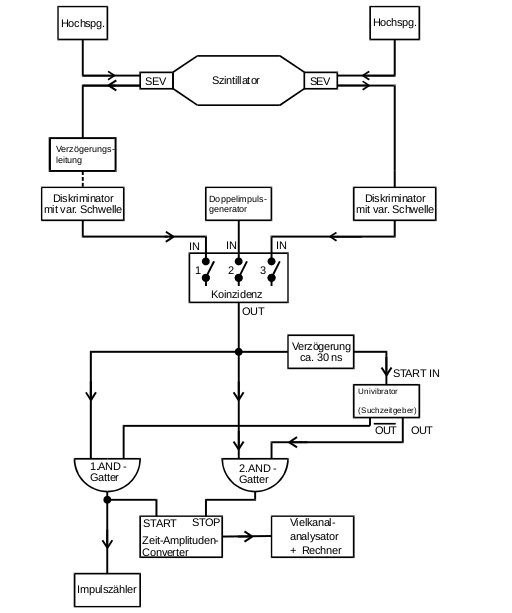
\includegraphics[width=0.8\linewidth,height=0.8\textheight,keepaspectratio]{Bilder/block.png}
	\caption{Blockschaltbild der Messapparatur \cite{Anl}}
	\label{FIG:Aufbau}
\end{figure}

\subsection{Justage}
Da die beiden SEV unterschiedliche elektrische Eigenschaften besitzen werden zunächst Verzögerungsleitungen einjustiert, sodass die Ausgangsrate nach der Koinzidenzschaltung maximal ist. Anschließend werden die Schwellwerte der Diskriminatoren einjustiert und die Suchzeit über den Univibrator eingestellt. Danach wird eine Kalbibration der Zeitachse vorgenommen und die Messung begonnen.

\section{Auswertung}

\subsection{Verzögerungsleitung}
Zunächst muss die Verzögerungsleitung so eingestellt werden, dass von Signale, die von beiden SEVs gemessen wurden, auch nahezu gleichzeitig in der Koinzidenzschaltung ankommen. Es wird dazu die Verzögerung im ns Bereich variiert und die Zählrate grafisch dargestellt. Die optimale Verzögerung liegt im Maximum der Zählrate.

\begin{figure}[htbp]
	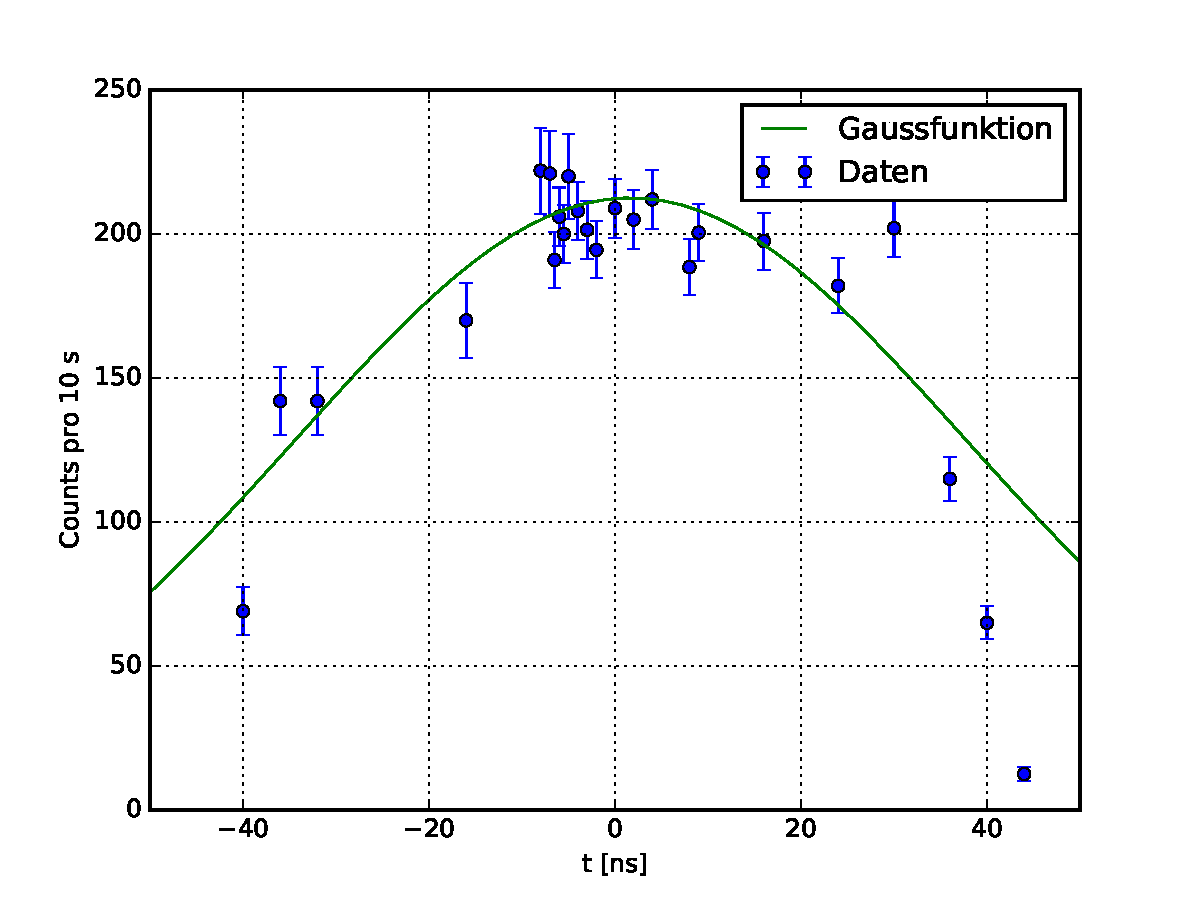
\includegraphics[width=0.8\textwidth]{./Bilder/koinzidenz.pdf}
	\caption{Zählrate gegen die zeitliche Verzögerung der Signale aufgetragen. Der maximale Wert wird durch den Fit einer Gaussfunktion ermittelt.}
	\label{fig:koinzidenz}
\end{figure}

Die gemessene Verteilung ist in Abbildung \ref{fig:koinzidenz} dargestellt. Die Zählrate hat ein sehr breites Maximum. Der Fit einer Gausschen Normalverteilung
\begin{align}
	f(x,\mu,\sigma) = A\cdot e^{-\frac{(x-\mu)^2}{\sigma^2}}
\end{align}
ergab:
\begin{align}
A &= (233.69 \pm 46.4)\,\text{Counts}\\
\mu &= (-3.07 \pm 1.3)\,\si{ns}\\
\sigma &= ({21.32} \pm 3.40)\,\si{\text{Counts}}
\end{align}

Für die Messung wurde eine Verzögerung von -4\,\si{ns} gewählt, da die Zählrate bei dieser Einstellung am größten war. Dieser Wert sollte das Ergebnis jedoch nicht beeinflussen, da er noch innerhalb der 1$\sigma$-Umgebung liegt.

Anschließend wurde der Threshold des Univibrators so eingestellt, dass die Anfängliche Zählrate von etwa 50 Counts/s auf 25 Counts/s absinkt. Letzterer Wert entspricht in etwa der theoretisch erwarteten Zählrate von kosmischen Myonen auf die Fläche des Detektortankes bezogen.

\subsection{Eichung des Vielkanal-Analysators}
Der Zeit-Amplituden-Konverter wandelt die Zeitdifferenz zwischen dem Start- und dem Stopsignal in eine Spannung um, die vom Vielkanalanalysator ausgelesen wird. Um den Zusammenhang zwischen Zeitdifferenz und Kanal zu erhalten, wird die Schaltung mit Sinusimpulsen betrieben, deren Abstand durch den Doppelimpulsgenerator vorgegeben wurden. Wenn eine Zeitdifferenz auf mehrere direkt nebeneinander liegende Kanäle abgebildet wurde, so wurde als Kanal der gewichtete Mittelwert gewählt. Die Zeitdifferenz wird in 1\,\si{ns} Schritten von 1\,ns bis 9\,ns variiert und gegen die Channel ID in \mbox{Abbildung \ref{fig:linFit}} aufgetragen.

\begin{figure}[H]
	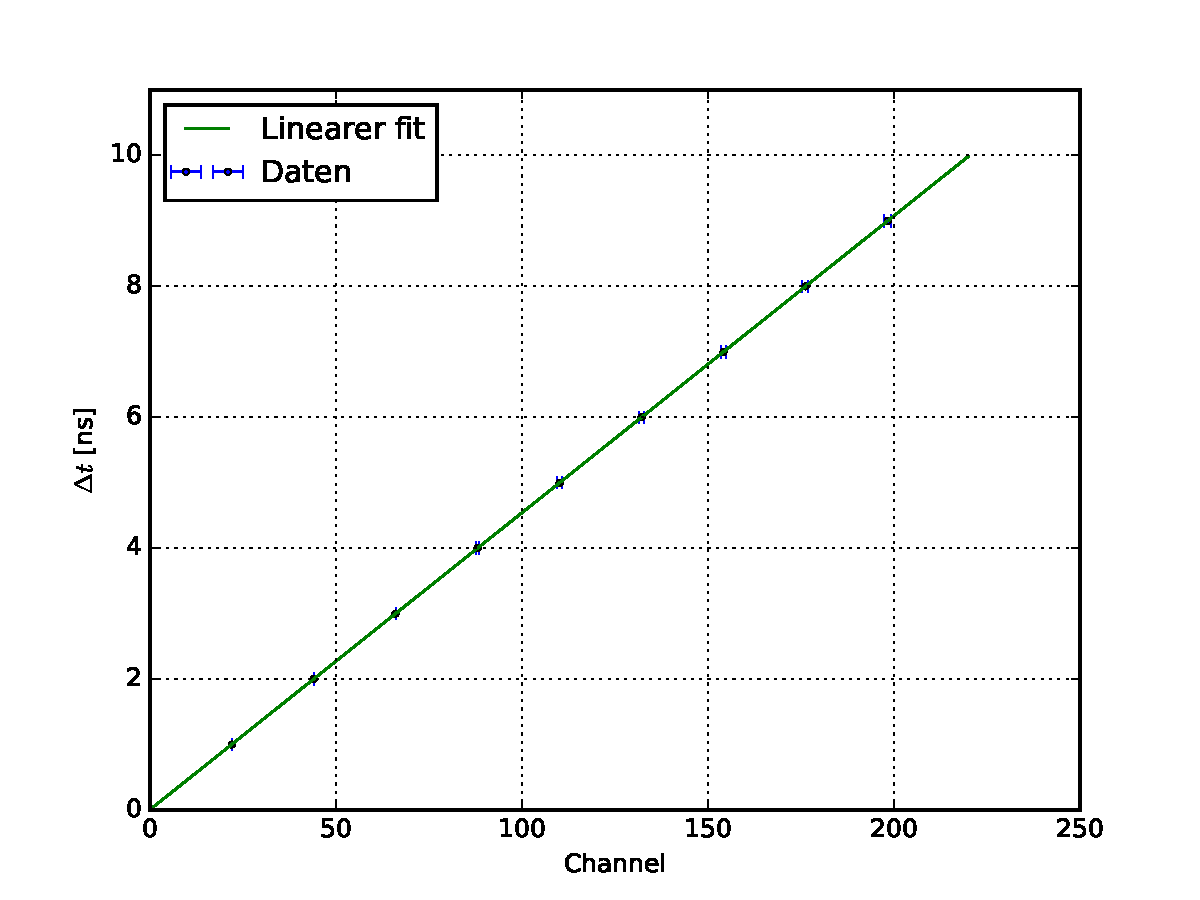
\includegraphics[width=0.8\textwidth]{./Bilder/linFit.pdf}
	\caption{Zeitdifferenz aus dem Doppelpulsgenerator gegen die Channel ID des Vielkanal-Analysators aufgetragen. Der Verlauf entspricht dem einer Geraden.}
	\label{fig:linFit}
\end{figure}

Als Fitfunktion wurde eine Gerade der Form
\begin{align}
	f(x) = mx + b
\end{align}
verwendet. Der Fit ergab folgende Werte für die Parameter:
\begin{align}
	m = 0.045 \pm 2.64\cdot10^{-10}\\
	b = 0.0055 \pm 4.08 \cdot 10^{-6}
\end{align}

\subsection{Die Lebensdauer von Myonen}
Entsprechend des zuvor ermittelten Zusammenhanges zwischen Kanal und Zeitdifferenz kann nun für die Durchgeführte Messung die Aufenthaltsdauer der Myonen im Detektortank in Abbildung \ref{fig:lebensdauer} visualisiert werden.

\begin{figure}[htbp]
	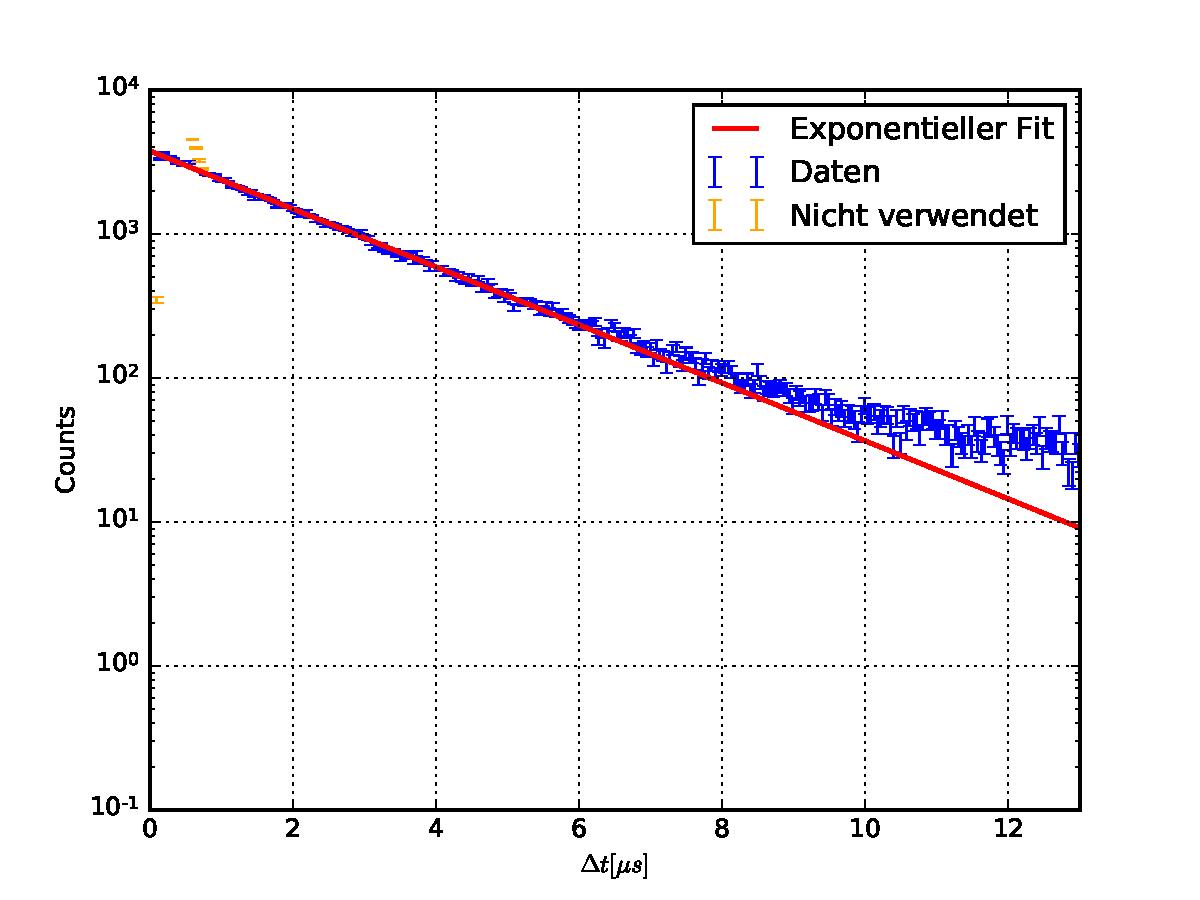
\includegraphics{./Bilder/lebensdauer.pdf}
	\caption{Messwerte der kosmischen Myonen und an die Messwerte gefittete Exponentialfunktion.}
	\label{fig:lebensdauer}
\end{figure}

Als Verteilung wurde eine Exponentialverteilung entsprechend Gleichung \ref{eqn:WSK4} zugrunde gelegt. Der Fit ergibt für die mittlere Lebenszeit
\begin{align}
	\tau = \frac{1}{\lambda} = (1.99 \pm 0.028)\,\text{$\mu$s}
\end{align}
und für den konstanten Untergrund
\begin{align}
c = 4.28 \pm 126.39\,\text{Counts}
\end{align}

\section{Diskussion}
Es gelang mit der Apparatur den Zerfall von Myonen im Detektortank nachzuweisen. Die mittlere Lebensdauer von 1.99\,\si{\micro \second} liegt unterhalb des Literatur Werts von etwa 2.2\,\si{\micro\second}. Diese Abweichung könnte dadurch erklärt werden, dass der Threshold des Univibrators möglicherweise noch höher eingestellt werden muss. Wahrscheinlicher ist es jedoch, dass das Szintilatormedium die Lebensdauer der Myonen in Vakuum deutlich merklich reduziert.

Für den Peak in den Zählraten bei etwa 1\,\si{\micro\second} sowie den plötzlichen Abfall der Zählrate bei etwa 13\,\si{\micro\second} wurde keine Erklärung gefunden. Insbesondere letzterer macht sich in dem großen Fehler der Untergrund-Rate bemerkbar.

\clearpage
\begin{thebibliography}{WissOnl}
\bibitem{Anl} TU Dortmund Versuchsanleitung zu Versuch Nr.01 (abgerufen am 20.6.2014) \url{http://129.217.224.2/HOMEPAGE/PHYSIKER/BACHELOR/FP/SKRIPT/V01.pdf}

\bibitem{PDG} Particle Data Group. Particle physics booklet. Institute of Physics publishing, 2006.

\end{thebibliography}
\end{document}
